%%%%%%%%%%%%%%%%%%%%%%%%%%%%%%%%%%%%%%%%%%%%%%%%%%%
% DECLARATION DE LA CLASSE DU DOCUMENT
%%%%%%%%%%%%%%%%%%%%%%%%%%%%%%%%%%%%%%%%%%%%%%%%%%%
%% Utiliser le format suivant:
% \documentclass[type de papier% ("letterpaper" demandé)
% , simple ou recto verso% ("oneside" ou "twoside")%
% , taille de la police% ("12pt" demandé)%
% , type de document% ("these", "memoire", "memoireprojet" ou "thesepararticles")%
% , langue du document ("francais" ou "english")%
% , options supplémentaires% ("creativecommons" pour préciser que le document est soumis à la licence créative commomns, "hyperref", "withAlgo2e" pour utiliser le package algorithm2e avec la mise en page correcte de la liste des algorithmes)
%]{thETS}

%% Exemple pour une thèse creative commons, utilisant le package hyperref
\documentclass[letterpaper%
, twoside%
, 12pt%
,these%
,francais
,creativecommons,hyperref%
]{thETS}

%%%%%%%%%%%%%%%%%%%%%%%%%%%%%%%%%%%%%%%%%%%%%%%%%%%
% IMPORTANT: NOTES D'IMPRESSION POUR RESPECTER LES MARGES
%%%%%%%%%%%%%%%%%%%%%%%%%%%%%%%%%%%%%%%%%%%%%%%%%%%
%%  Si vous créez un fichier PDF directement avec PDFLatex, et vous utilisez Acrobat Reader
%% pour faire l'impression, n'oubliez-pas de changer l'option <<Mise à l'échelle>> pour la valeur
%% <<Aucune>> pour que les marges soient imprimés correctement.
%%%%%%%%%%%%%%%%%%%%%%%%%%%%%%%%%%%%%%%%%%%%%%%%%%%


%%%%%%%%%%%%%%%%%%%%%%%%%%%%%%%%%%%%%%%%%%%%%%%%%%%
% DECLARATION D'UNE LISTE DE RÉFÉRENCES SUPPLÉMENTAIRE
%%%%%%%%%%%%%%%%%%%%%%%%%%%%%%%%%%%%%%%%%%%%%%%%%%%
%% Exemple de création d'une liste de références en plus de la liste bibliographique
% "refs" est utilisé en suffixe des commandes de citation de de bibliogtraphie
\newcites{refs}{LISTE DE RÉFÉRENCES}

%%%%%%%%%%%%%%%%%%%%%%%%%%%%%%%%%%%%%%%%%%%%%%%%%%%
% DECLARATION DES INFORMATIONS DE LA PAGE TITRE
%%%%%%%%%%%%%%%%%%%%%%%%%%%%%%%%%%%%%%%%%%%%%%%%%%%

\title{Titre du document}

\author{Prénom NOM DE FAMILLE}
\authorcopyright{Prénom Nom}

\datesoutenance{``Date de soutenance''}

\datedepot{``Date du dépôt au Bureau des cycles supérieurs''}

\directeur{M.}{Prénom Nom}{Nom du département et institution}

%\directeur{Mme.}{Prénom Nom}{Nom du département et institution}

\codirecteur{Mme.}{Prénom Nom}{département et institution}

%\codirecteurB{M.}{Prénom Nom}{département et institution}

\president{M.}{Prénom Nom}{département et institution}

\examinexterne{M.}{Prénom Nom}{département et institution}{}

%\jury{Mme.}{Prénom Nom}{département et institution}{}

%%%%%%%%%%%%%%%%%%%%%%%%%%%%%%%%%%%%%%%%%%%%%%%%%%%
% CHANGEMENT DE L'INTITULÉ DU DIPLOME
%%%%%%%%%%%%%%%%%%%%%%%%%%%%%%%%%%%%%%%%%%%%%%%%%%%
%% Il est possible de modifier l'intitulé du diplome en redéfinissant la commande
% \lediplome, comme dans l'exemple suivant:
%\renewcommand{\lediplome}{DE LA MAÎTRISE\\AVEC MEMOIRE EN GÉNIE ÉLECTRIQUE\\M. Sc. A.}

\listfiles

%%%%%%%%%%%%%%%%%%%%%%%%%%%%%%%%%%%%%%%%%%%%%%%%%%%
% DÉBUT DU DOCUMENT
%%%%%%%%%%%%%%%%%%%%%%%%%%%%%%%%%%%%%%%%%%%%%%%%%%%
\begin{document}

\pagenumbering{Roman}

%%- Affichage de la page titre -%%
\maketitle

%%- Affichage de la présentaiton du jury -%%
\presentjury

%%%- Avant propos -%%
\begin{avantpropos}

\lipsum[1] % Texte de remplissage pour donner un exemple de la mise en page

\end{avantpropos}



%%- Remerciements -%%
\begin{remerciements}

\lipsum[1] % Texte de remplissage pour donner un exemple de la mise en page


\end{remerciements}


%%- Sommaire -%%

\begin{sommaire}{mot-clé1, mot-clé2}

\lipsum[1] % Texte de remplissage pour donner un exemple de la mise en page

\end{sommaire}


%%- Abstract -%%
\begin{abstract}{Titre en anglais}{keyword1, keyword2}

\lipsum[1] % Texte de remplissage pour donner un exemple de la mise en page

\end{abstract}


%%- Affichage de la table des matières -%%
\tableofcontents


%%- Affichage de la liste des tableaux -%%
\listoftables


%%- Affichage de la liste des Figures -%%
\listoffigures


%%- Déclaration et affichage de la liste des abbréviations -%%
\begin{listofabbr}[3cm]
\item [ETS] École de Technologie Supérieure
\item [ASC] Agence Spatiale Canadienne
\end{listofabbr}


%%- Déclaration et affichage de la liste des symboles -%%
\begin{listofsymbols}[3cm]
\item [a] Première lettre de l'alphabet
\item [A] Première lettre de l'alphabet en majuscule
\end{listofsymbols}


\cleardoublepage

\pagenumbering{arabic}

% Marginpar à gauche du document
\reversemarginpar

%%%%%%%%%%%%%%%%%%%%%%%%%%%%%%%%%%%%%%%%%%%%%%%%%%%
% EXEMPLE DE CORPS DE THÈSE OU MÉMOIRE
%%%%%%%%%%%%%%%%%%%%%%%%%%%%%%%%%%%%%%%%%%%%%%%%%%%

\begin{introduction}

\lipsum[1] % Texte de remplissage pour donner un exemple de la mise en page

% Exemple de déclaration de figure
\begin{figure}
	\centering % Les figures doivent être centrées
	\fbox{ % Les figures doivent être délimitées par un rectangle
		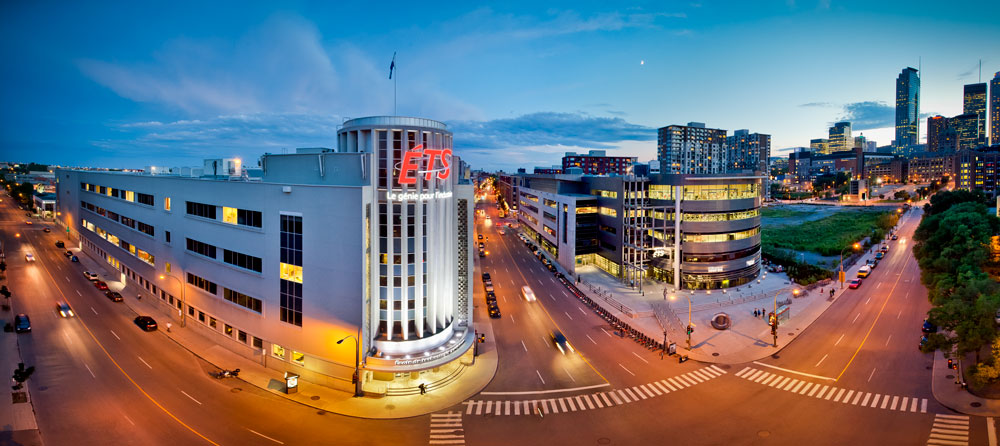
\includegraphics[width=0.75\textwidth]{Figures/vueEts.jpg} % Spécification du paramètres "width", la largeur de l'image (en conservant les proportions). La largeur est ici restreinte à 0.75 fois "\textwidth", qui est la largeur maximale du texte dans le document en prenant en compte les marges
	}
	 \\ \parbox{0.75\textwidth}{\caption{Test de longue légende, avec utilisation de framebox et parbox pour restreindre la largeur de la légende.}\label{fig:vueEts}} % Utilisation d'une parbox pour restreindre la largeur de la légende. Ici la taille maximale a été fixée à la largeur choisie pour l'image (0.75\textwidth). Le décanat demande d'éviter d'avoir des légendes qui dépasse les figures, dans la mesure du possible (si l'image est trop petite, la légende peut dépasser sa largeur).
\end{figure}

\lipsum[1] % Texte de remplissage pour donner un exemple de la mise en page


\end{introduction}

%%- Décommenter pour chapitre revue de littérature, pour les thèses par article -%%
%\begin{revuedelitterature}

%\end{revuedelitterature}

%%- Premier chapitre de démonstration -%%
\chapter{Test de long titre de Chapitre, avec retour à la ligne. Lorem ipsum dolor sit amet, consectetur adipiscing elit. Pellentesque justo justo, porta sagittis feugiat eget, ornare rhoncus ligula. Nunc non odio sed lacus rutrum rhoncus.}


\section{Tests de mise en page}

Dans cette section, différents environnements de mise en page sont présentés.

\subsection{Test des listings}

Présentation des principaux listings: les énumations et les listes.


\subsubsection{Énumérations: environement enum}

Test de l'environment enum:
\begin{enumerate}
 \item test 1
 \item test 2
\end{enumerate}

\subsubsection{Listes: environement itemize}

Test de l'environement itemize
\begin{itemize}
 \item test 1
 \item test 2
\end{itemize}

\subsection{Test des équations}

Mise en page des équations

\begin{equation}
   \beta = 8
\end{equation}

\begin{equation}
   \bm{\gamma} = \alpha \times 3
\end{equation}

\section{Seconde section}

Exemple de seconde section pour illustrer la mise en page de la table des matières


%%- Deuxiemme chapitre de démonstration -%%
\chapter{Ajout d'un second chapitre}

\section{Test de mise en page d'un tableau}

Les tableaux sont soumis aux mêmes contraintes que les figures, en dehors de la position de la légende qui doit être au dessus.


\begin{table}
		\parbox{0.65\textwidth}{\caption{Test de longue légende pour un tableau, avec retour à la ligne.}} % Contrainte manuelle de la largeur de la légende
		\begin{tabular}{|c|c|c|c|c|c|c|c|}
		\hline
			{\bf titre} & {\bf titre} & {\bf titre} & {\bf titre} & {\bf titre} & {\bf titre} & {\bf titre} & {\bf titre} \\
	  \hline
			blá & blá & blá & blá & blá & blá & blá & blá \\
	  \hline
			blá & blá & blá & blá & blá & blá & blá & blá \\
	  \hline
			blá & blá & blá & blá & blá & blá & blá & blá \\
	  \hline
			blá & blá & blá & blá & blá & blá & blá & blá \\
	  \hline
			blá & blá & blá & blá & blá & blá & blá & blá \\
	  \hline
			blá & blá & blá & blá & blá & blá & blá & blá \\
	  \hline
		\end{tabular}
\end{table}


\section{Test des références}

\subsection{Références à la bibliographie}

Citation d'une référence de la bibliographie \citep{BookExample}.

\subsection{Références à la liste de références "refs"}

Citation d'une référence de la liste de référence "refs" déclarée au début du document \citerefs{Test}.

\subsection{Références à un label du document}

Référence à une Figure associée à un label: Figure \ref{fig:vueEts}.

\subsection{Références à des adresses}

\subsubsection{Test de href}

Utilisation de href, pour intégrer un lien dans une portion de texte:
\href{http://www.etsmtl.ca/Etudiants-actuels/Cycles-sup/Realisation-etudes/Guides-gabarits}{Lien vers la page des gabarits de l'ÉTS}.

\subsubsection{Test de url}

Utilisation de url pour citer un lien cliquable:
\url{http://www.etsmtl.ca/Etudiants-actuels/Cycles-sup/Realisation-etudes/Guides-gabarits}.

%%- Troisième chapitre de démonstration -%%
\chapter{Exemple de thèse par articles intégrés}

% Utilisation de \articleAuthors{Noms}{Affiliations} pour affichier les auteurs de l'article et leur affiliation. Noms doit être sous la forme {Nom1 Prenom1}{Nom2 Prenom2}... , ainsi que les affiliations.
%Exemple \articleAuthors{{Nom1 Prenom1}}{{Affiliation 1}}

\articleAuthors{
{Prenom Nom\up{1}}{Prenom Nom\up{1}}
}{
{\up{1} Département de Génie Mécanique, École de Technologie Supérieure,\\
1100 Notre-Dame Ouest, Montréal, Québec, Canada H3C 1K3
\\~\\
Article soumis à la revue « Vecteur environnement » en septembre 2010.}
}

\section{Section 1}

\lipsum[1]

%%- Conclusion -%%
\begin{conclusion}

\lipsum[1] % Texte de remplissage pour donner un exemple de la mise en page

\end{conclusion}


%%%%%%%%%%%%%%%%%%%%%%%%%%%%%%%%%%%%%%%%%%%%%%%%%%%
%  EXEMPLE D'ANNEXE:
%%%%%%%%%%%%%%%%%%%%%%%%%%%%%%%%%%%%%%%%%%%%%%%%%%%
\appendix

%% Lorsqu'on a plus qu'une annexe.
\multiannexe

%% Inclusion d'une annexe externe
% \include{extAnnex}

\chapter{Test d'une annexe}


\section{Première Section de l'Annexe}


\subsection{Figures en annexe}

\begin{figure}
	\centering
	\fbox{
		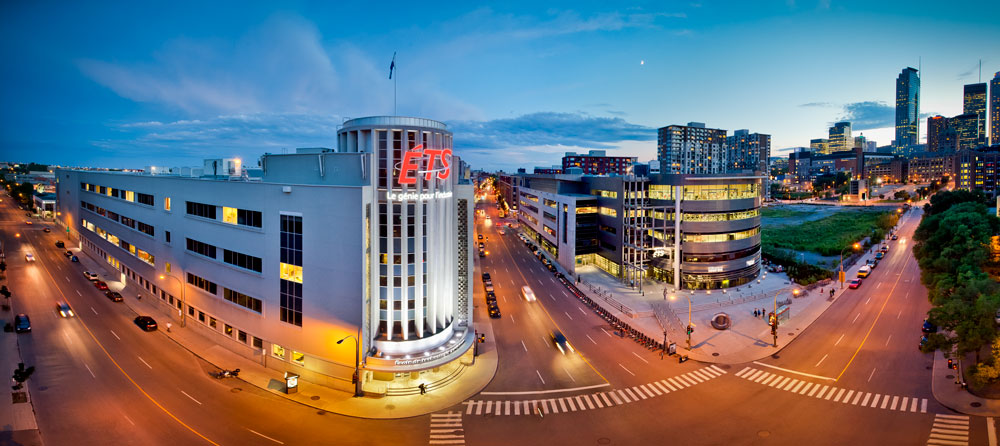
\includegraphics[width=0.75\textwidth]{Figures/vueEts.jpg}
	}
	 \\ \parbox{0.75\textwidth}{\caption{Figure en Annexe.}\label{fig:testAp}}
\end{figure}

Les figures en annexe se déclarent de la même manière que dans le reste du document, et leur numération est automatiquement adaptée (exemple, Figure \ref{fig:testAp}).

\subsubsection{Tables en annexe}

\begin{table}
		\parbox{0.65\textwidth}{\caption{Table en Annexe.}\label{tab:testAp}}

		\begin{tabular}{|c|c|c|c|c|c|c|c|}
		\hline
			{\bf titre} & {\bf titre} & {\bf titre} & {\bf titre} & {\bf titre} & {\bf titre} & {\bf titre} & {\bf titre} \\
	  \hline
			blá & blá & blá & blá & blá & blá & blá & blá \\
	  \hline
			blá & blá & blá & blá & blá & blá & blá & blá \\
	  \hline
			blá & blá & blá & blá & blá & blá & blá & blá \\
	  \hline
			blá & blá & blá & blá & blá & blá & blá & blá \\
	  \hline
			blá & blá & blá & blá & blá & blá & blá & blá \\
	  \hline
			blá & blá & blá & blá & blá & blá & blá & blá \\
	  \hline
		\end{tabular}
\end{table}

Même chose pour les tableaux (exemple, Tableau \ref{tab:testAp}).


%%%%%%%%%%%%%%%%%%%%%%%%%%%%%%%%%%%%%%%%%%%%%%%%%%%
% BIBLIOGRAPHIE ET RÉFÉRENCES
%%%%%%%%%%%%%%%%%%%%%%%%%%%%%%%%%%%%%%%%%%%%%%%%%%%

%%- Bibliographie -%%
\newpage
%Interligne sinmple pour la bibliographie
\begin{spacing}{1}
	\nocite{*} % Utiliser la commande nocite pour afficher des références qui n'ont pas été citées dans le document. '*' permet de toutes les afficher.
	\bibliographystyle{bibETS} % Utilisation du style bibliographique de l'ETS
	\addcontentsline{toc}{chapter}{BIBLIOGRAPHIE} % Ajout de la bibliographie à la table des matières

	\bibliography{biblio_fr} % Liste des fichiers bib de bibliographie, biblio.bib est un exemple

\end{spacing}

%%- Références, exemple des références "refs" --%
%%%%%%%%%%%%%%%%%%%%%%%%%%%%%%%%%%%%%%%%%%%%%%%%%%%
% IMPORTANT: NOTES POUR COMPILER ET AFFICHER LES RÉFÉRENCES ADDITIONNELLES (remplacer "refs" par le suffixe choisi)
%%%%%%%%%%%%%%%%%%%%%%%%%%%%%%%%%%%%%%%%%%%%%%%%%%%
% Suivre les trois étapes:
%   1. Compiler le document une fois pour renseigner les références utilisées dans refs.aux
%   2. Lancer la compilation des références
% 		- Sous Linux: Utilser la commande "bibtex refs" dans le dossier du document
%		- Sous MacOSX (distribution MacTex): Utilser la commande "/usr/texbin/bibtex refs" dans le dossier du document
%		- Sous Windows: Éditer le script "update_refs.bat" pour renseigner le bon suffixe, et le lancer
%   3. Recompiler le document deux fois
%%%%%%%%%%%%%%%%%%%%%%%%%%%%%%%%%%%%%%%%%%%%%%%%%%%

\newpage
% Le fonctionnement est similaire, en rajoutant le suffixe choisi "refs" à la fin de chaque commande de bibliographie
\begin{spacing}{1}
	%\nociterefs{*}
	\bibliographystylerefs{bibETS}
	\addcontentsline{toc}{chapter}{LISTE DE RÉFÉRENCES}

	\bibliographyrefs{refs} % Liste des fichiers bib de référence, refs.bib est un exemple

\end{spacing}

\end{document}
